%%%%%%%%%%%%%%%%%%%%%%%%%%%%%%%%%%%%%%%%%%%%%%%%%%%%%%%%%%%%%%%%%%%%%%%%%%%%%%%%%%
\begin{frame}[fragile]\frametitle{}
\begin{center}
{\Large Introduction to Ayurveda}
\end{center}
\end{frame}

%%%%%%%%%%%%%%%%%%%%%%%%%%%%%%%%%%%%%%%%%%%%%%%%%%%%%%%%%%%
\begin{frame}[fragile]\frametitle{History}
	\begin{itemize}
	\item  Roughly 5000 years old
	\item आयुर्वेद Meaning: life आयु:, knowledge(वेद)
	\end{itemize}

\end{frame}

%%%%%%%%%%%%%%%%%%%%%%%%%%%%%%%%%%%%%%%%%%%%%%%%%%%%%%%%%%%
\begin{frame}[fragile]\frametitle{Medicine Systems}
	\begin{itemize}
	\item Modern Medicine: Allopathy, emergency
	\item  Traditional Chinese Medicine: Moving energies
	\item Indian Ayurvedic Medicine: Includes Spiritual apart from Physical and Mental.
	\end{itemize}

\end{frame}

%%%%%%%%%%%%%%%%%%%%%%%%%%%%%%%%%%%%%%%%%%%%%%%%%%%%%%%%%%%
\begin{frame}[fragile]\frametitle{Benefits}
	\begin{itemize}
	\item Integrated-Holistic Science
	\item Not just corrective but preventive as well
	\item Life style prescriptions
	\end{itemize}

\end{frame}

%%%%%%%%%%%%%%%%%%%%%%%%%%%%%%%%%%%%%%%%%%%%%%%%%%%%%%%%%%%
\begin{frame}[fragile]\frametitle{Principles}

\begin{center}
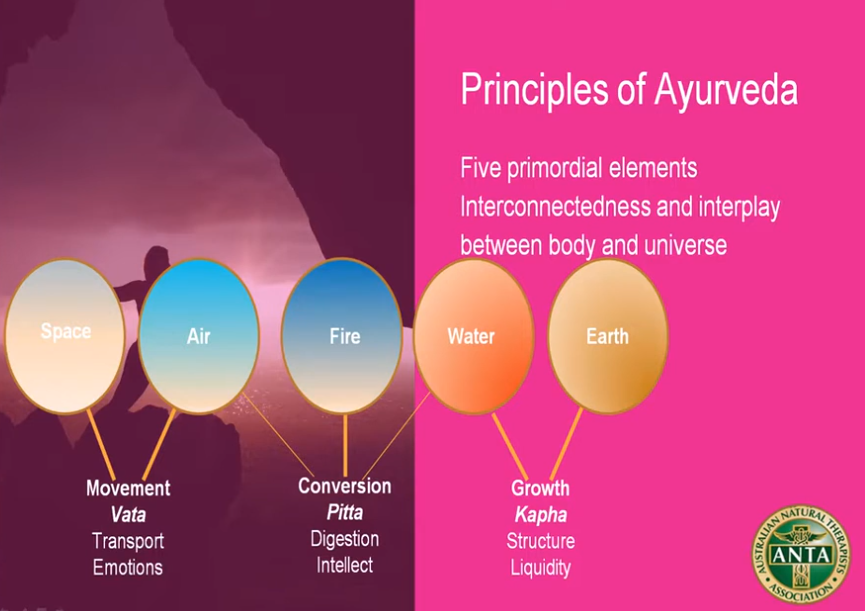
\includegraphics[width=0.7\linewidth,keepaspectratio]{images/ayur1}
\end{center}

{\tiny (Ref: Ayurvedic Concepts with Neerja Ahuja - ANTA seminar 2017)}

\end{frame}

%%%%%%%%%%%%%%%%%%%%%%%%%%%%%%%%%%%%%%%%%%%%%%%%%%%%%%%%%%%
\begin{frame}[fragile]\frametitle{Disease}

\begin{center}
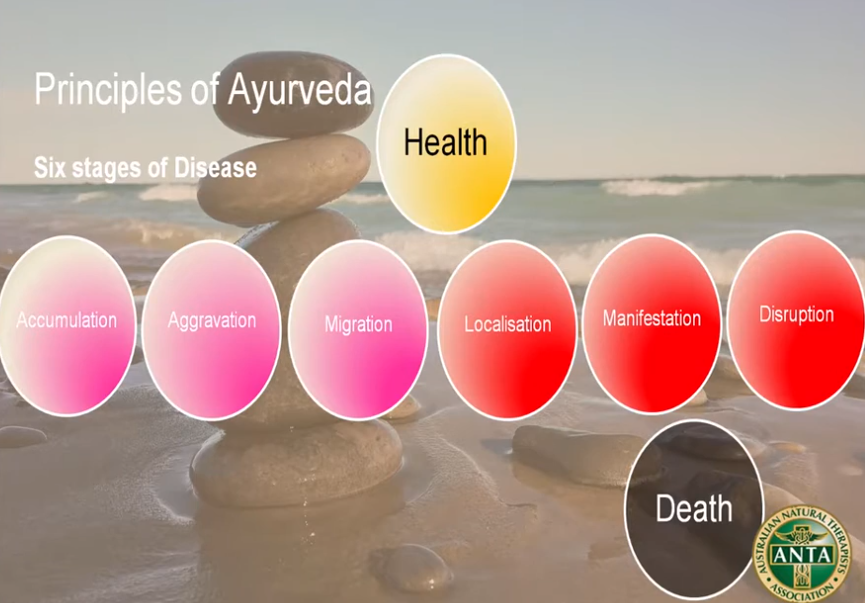
\includegraphics[width=0.7\linewidth,keepaspectratio]{images/ayur2}
\end{center}

{\tiny (Ref: Ayurvedic Concepts with Neerja Ahuja - ANTA seminar 2017)}

\end{frame}

%%%%%%%%%%%%%%%%%%%%%%%%%%%%%%%%%%%%%%%%%%%%%%%%%%%%%%%%%%%
\begin{frame}[fragile]\frametitle{Goals of Life}

	\begin{itemize}
	\item  अर्थ Prosperity, earnings, career
	\item  काम Pleasures, hobbies,relationships
	\item  धर्म Duty, responsibilities
	\item  मोक्ष Liberation
	\end{itemize}

\end{frame}

%%%%%%%%%%%%%%%%%%%%%%%%%%%%%%%%%%%%%%%%%%%%%%%%%%%%%%%%%%%
\begin{frame}[fragile]\frametitle{Pillars of Life}

	\begin{itemize}
	\item  आहार Food, Digestion
	\item  निद्रा Sleep, rest
	\item  ब्र्ह्मचर्य Sexual restraint
	\end{itemize}

\end{frame}

%%%%%%%%%%%%%%%%%%%%%%%%%%%%%%%%%%%%%%%%%%%%%%%%%%%%%%%%%%%
\begin{frame}[fragile]\frametitle{Body levels}
	\begin{itemize}
	\item  Physical body : 5 elements (पृथ्वी जल वायु अग्नि आकाश)
	\item Subtle body: Mind
	\item Casual body: Karma
	
	\end{itemize}

\end{frame}

%%%%%%%%%%%%%%%%%%%%%%%%%%%%%%%%%%%%%%%%%%%%%%%%%%%%%%%%%%%
\begin{frame}[fragile]\frametitle{Layers of Existence}
	\begin{itemize}
	\item अन्नमय कोष Physical body 
	\item प्राणमय कोष Subtle body for sense of heat, cold, hunger and thirst
	\item मनोमय कोष Subtle body for personality, emotions, intuition
	\item विज्ञानमय कोष Subtle body for intellect, ego.
	\item आनन्दमय कोष  Causal body for Bliss, realization.
	\end{itemize}

\end{frame}

%%%%%%%%%%%%%%%%%%%%%%%%%%%%%%%%%%%%%%%%%%%%%%%%%%%%%%%%%%%
\begin{frame}[fragile]\frametitle{States of Mind}

\begin{center}
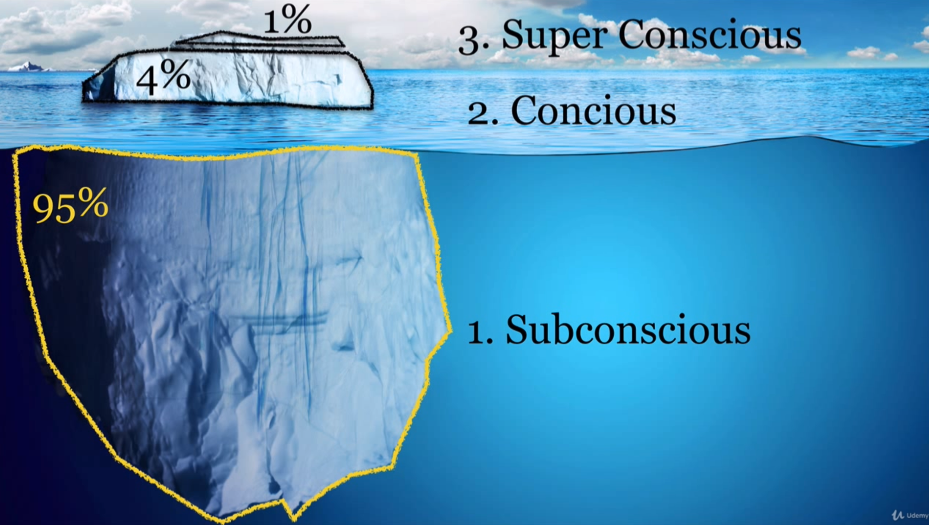
\includegraphics[width=\linewidth,keepaspectratio]{images/mind1}
\end{center}

{\tiny (Ref: Ayurvedic Basics - Udemy)}

\end{frame}

%%%%%%%%%%%%%%%%%%%%%%%%%%%%%%%%%%%%%%%%%%%%%%%%%%%%%%%%%%%
\begin{frame}[fragile]\frametitle{Subconscious Mind}
	\begin{itemize}
	\item Instincts
	\item Senses
	\item Lower emotions
	\item Past Experiences
	\end{itemize}
\end{frame}

%%%%%%%%%%%%%%%%%%%%%%%%%%%%%%%%%%%%%%%%%%%%%%%%%%%%%%%%%%%
\begin{frame}[fragile]\frametitle{Conscious Mind}
	\begin{itemize}
	\item Present moment
	\item Intellect
	\item Higher emotions
	\end{itemize}
\end{frame}


%%%%%%%%%%%%%%%%%%%%%%%%%%%%%%%%%%%%%%%%%%%%%%%%%%%%%%%%%%%
\begin{frame}[fragile]\frametitle{Super conscious Mind}
	\begin{itemize}
	\item Intuition
	\item Cosmic message
	\item Wake up from तमस, calm down रजस, nourish सत्त्व so that innermost intuition can be accessed.
	\end{itemize}
\end{frame}


%%%%%%%%%%%%%%%%%%%%%%%%%%%%%%%%%%%%%%%%%%%%%%%%%%%%%%%%%%%
\begin{frame}[fragile]\frametitle{Mechanics of Mind}
	\begin{itemize}
	\item You are not your mind.
	\item 5 senses bring signals to body (physical body)
	\item Breath connects body to mind (subtle body)
	\item Meditation connects mind to soul (causal body).
	\end{itemize}
\end{frame}



%%%%%%%%%%%%%%%%%%%%%%%%%%%%%%%%%%%%%%%%%%%%%%%%%%%%%%%%%%%
\begin{frame}[fragile]\frametitle{Body Types प्रक्रुति}
Based on imbalances (दोश)

	\begin{itemize}
	\item  Wind वात
	\item  Bile पित्त
	\item  Mucos कफ
	\item When the doshas are present in ``appropriate'' quantities, they support the health and integrity of the body
	\item When they are out of balance, they can cause illness and disease.
	\end{itemize}

\end{frame}

%%%%%%%%%%%%%%%%%%%%%%%%%%%%%%%%%%%%%%%%%%%%%%%%%%%%%%%%%%%
\begin{frame}[fragile]\frametitle{Wind वात}

	\begin{itemize}
	\item Made of: air and ether (sound energy medium)
	\item Governs: movement and communication.
	\item Characteristics: light, cold, dry, rough, mobile, subtle, and clear.	
	\item Likes Hot/warm surrounding
	\item Hands/feet are cold
	\item Quick to walk/talk/learn/forget.
	\item Good at art, music
	\item Prone to anxiety, stress, fear.
	\item Food to favor: Warm, moist, sweet, oily
	\item Food to avoid: dry, cold
	\end{itemize}

\end{frame}

%%%%%%%%%%%%%%%%%%%%%%%%%%%%%%%%%%%%%%%%%%%%%%%%%%%%%%%%%%%
\begin{frame}[fragile]\frametitle{Bile पित्त}

	\begin{itemize}
	\item Made of: fire, water
	\item Governs: transformation.
	\item Characteristics: light, sharp (or penetrating), hot, oily, liquid, and spreading.	
	\item Likes cold
	\item Forcefulness, passion
	\item Creative, sharp tongue/intellect
	\item Acidity, irritation, frustration
	\item Food to favor: cool
	\end{itemize}

\end{frame}


%%%%%%%%%%%%%%%%%%%%%%%%%%%%%%%%%%%%%%%%%%%%%%%%%%%%%%%%%%%
\begin{frame}[fragile]\frametitle{Mucos कफ}

	\begin{itemize}
	\item Made of: earth and water
	\item Governs: structure and cohesiveness.
	\item Characteristics: heavy, slow, cool, oily, smooth, dense, soft, stable, gross, and cloudy
	\item Stout, strong, slow talk/walk/learn/forget.
	\item Prone to weight gain, tumors
	\item Food to favor: light, dry
	\item Food to avoid: 	heavy, oily
	\end{itemize}

\end{frame}


%%%%%%%%%%%%%%%%%%%%%%%%%%%%%%%%%%%%%%%%%%%%%%%%%%%%%%%%%%%
\begin{frame}[fragile]\frametitle{Identify Body Type}

\begin{center}
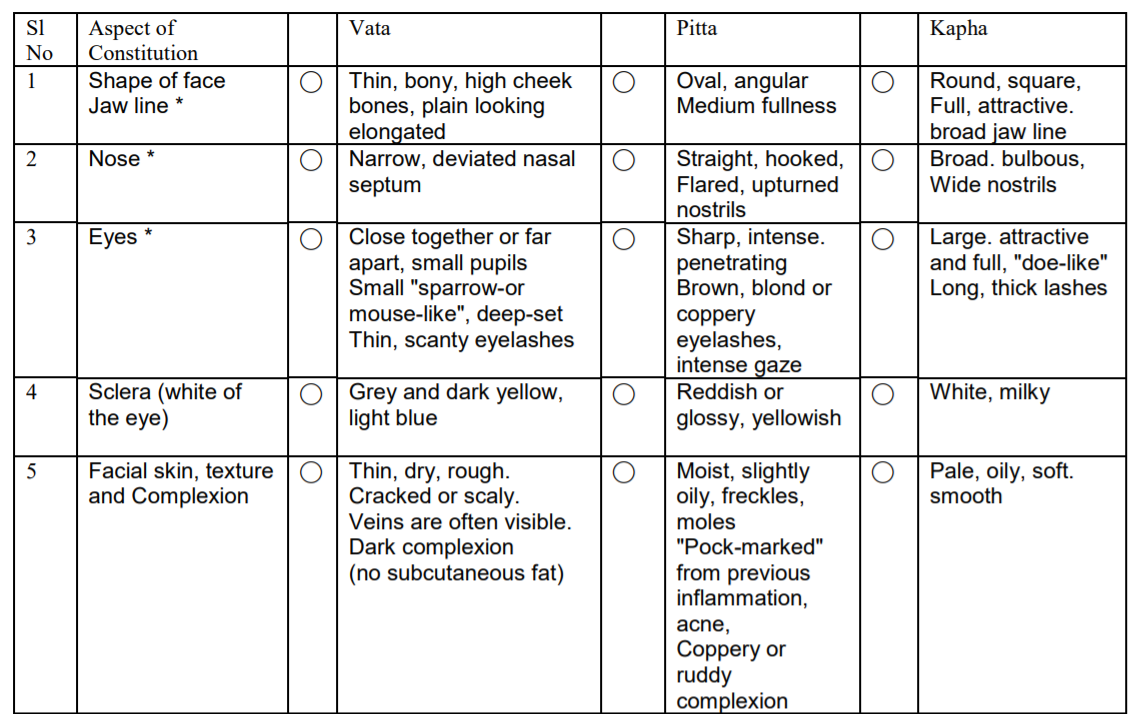
\includegraphics[width=\linewidth,keepaspectratio]{images/bt1}
\end{center}

{\tiny (Ref: Ayurveda Awareness Center, Udemy)}

\end{frame}


%%%%%%%%%%%%%%%%%%%%%%%%%%%%%%%%%%%%%%%%%%%%%%%%%%%%%%%%%%%
\begin{frame}[fragile]\frametitle{Identify Body Type}

\begin{center}
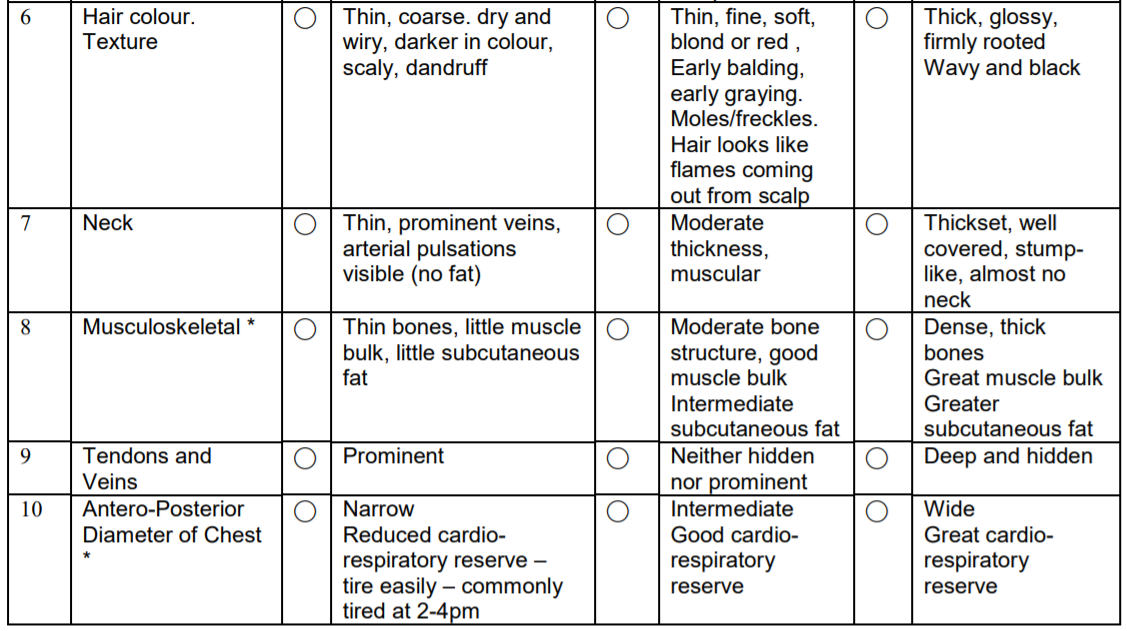
\includegraphics[width=\linewidth,keepaspectratio]{images/bt2}
\end{center}

{\tiny (Ref: Ayurveda Awareness Center, Udemy)}

\end{frame}


%%%%%%%%%%%%%%%%%%%%%%%%%%%%%%%%%%%%%%%%%%%%%%%%%%%%%%%%%%%
\begin{frame}[fragile]\frametitle{Identify Body Type}

\begin{center}
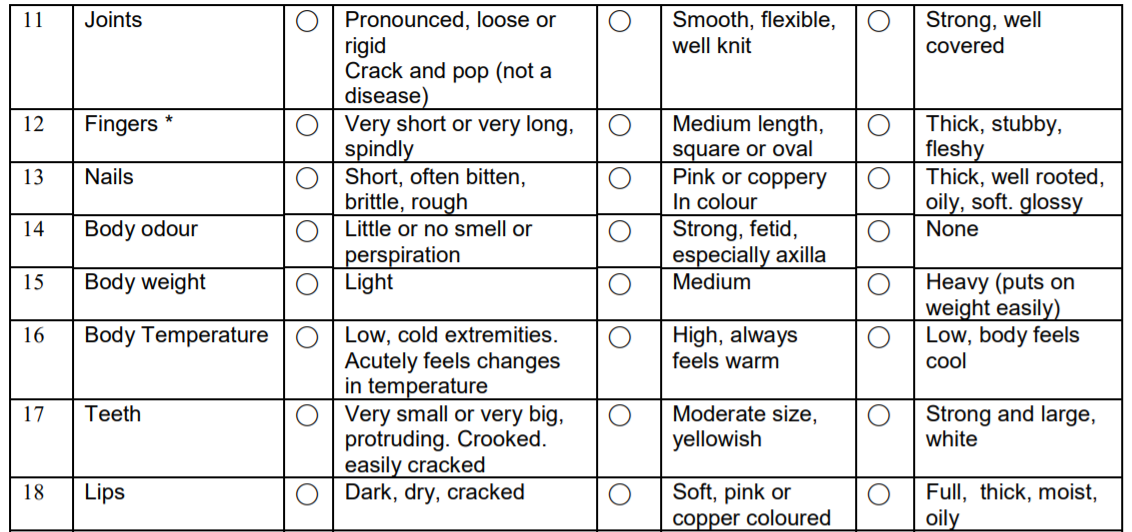
\includegraphics[width=\linewidth,keepaspectratio]{images/bt3}
\end{center}

{\tiny (Ref: Ayurveda Awareness Center, Udemy)}

\end{frame}


%%%%%%%%%%%%%%%%%%%%%%%%%%%%%%%%%%%%%%%%%%%%%%%%%%%%%%%%%%%
\begin{frame}[fragile]\frametitle{Identify Body Type}

\begin{center}
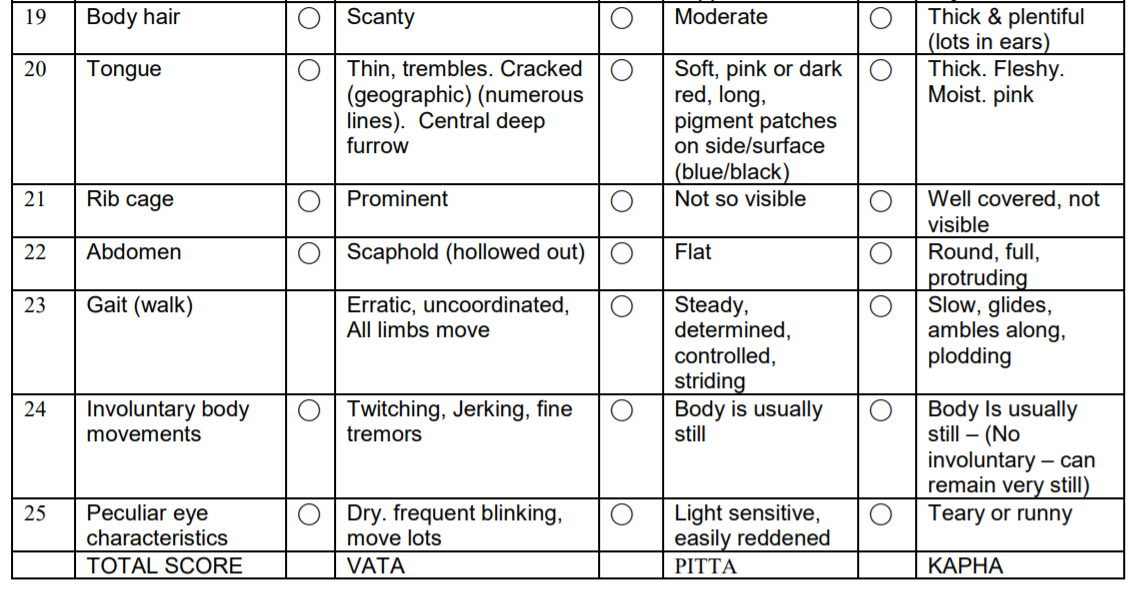
\includegraphics[width=\linewidth,keepaspectratio]{images/bt4}
\end{center}

{\tiny (Ref: Ayurveda Awareness Center, Udemy)}

\end{frame}

%%%%%%%%%%%%%%%%%%%%%%%%%%%%%%%%%%%%%%%%%%%%%%%%%%%%%%%%%%%
\begin{frame}[fragile]\frametitle{Stages in Life}

	\begin{itemize}
	\item  Everyone is born with a genetic disposition, ie one of the 3 body types.
	\item These get added by age-wise body types also.
	\item Childhood (0-15): कफ, tissues growing, increase body weight
	\item Adulthood (16-50): पित्त, competitiveness, acidity
	\item Old age (50+): वात, fears, nervousness, insomnia, gas
	\end{itemize}

\end{frame}

%%%%%%%%%%%%%%%%%%%%%%%%%%%%%%%%%%%%%%%%%%%%%%%%%%%%%%%%%%%
\begin{frame}[fragile]\frametitle{Stages in a Day}

One of the 3 body types is predominant at different times in a day

\begin{center}
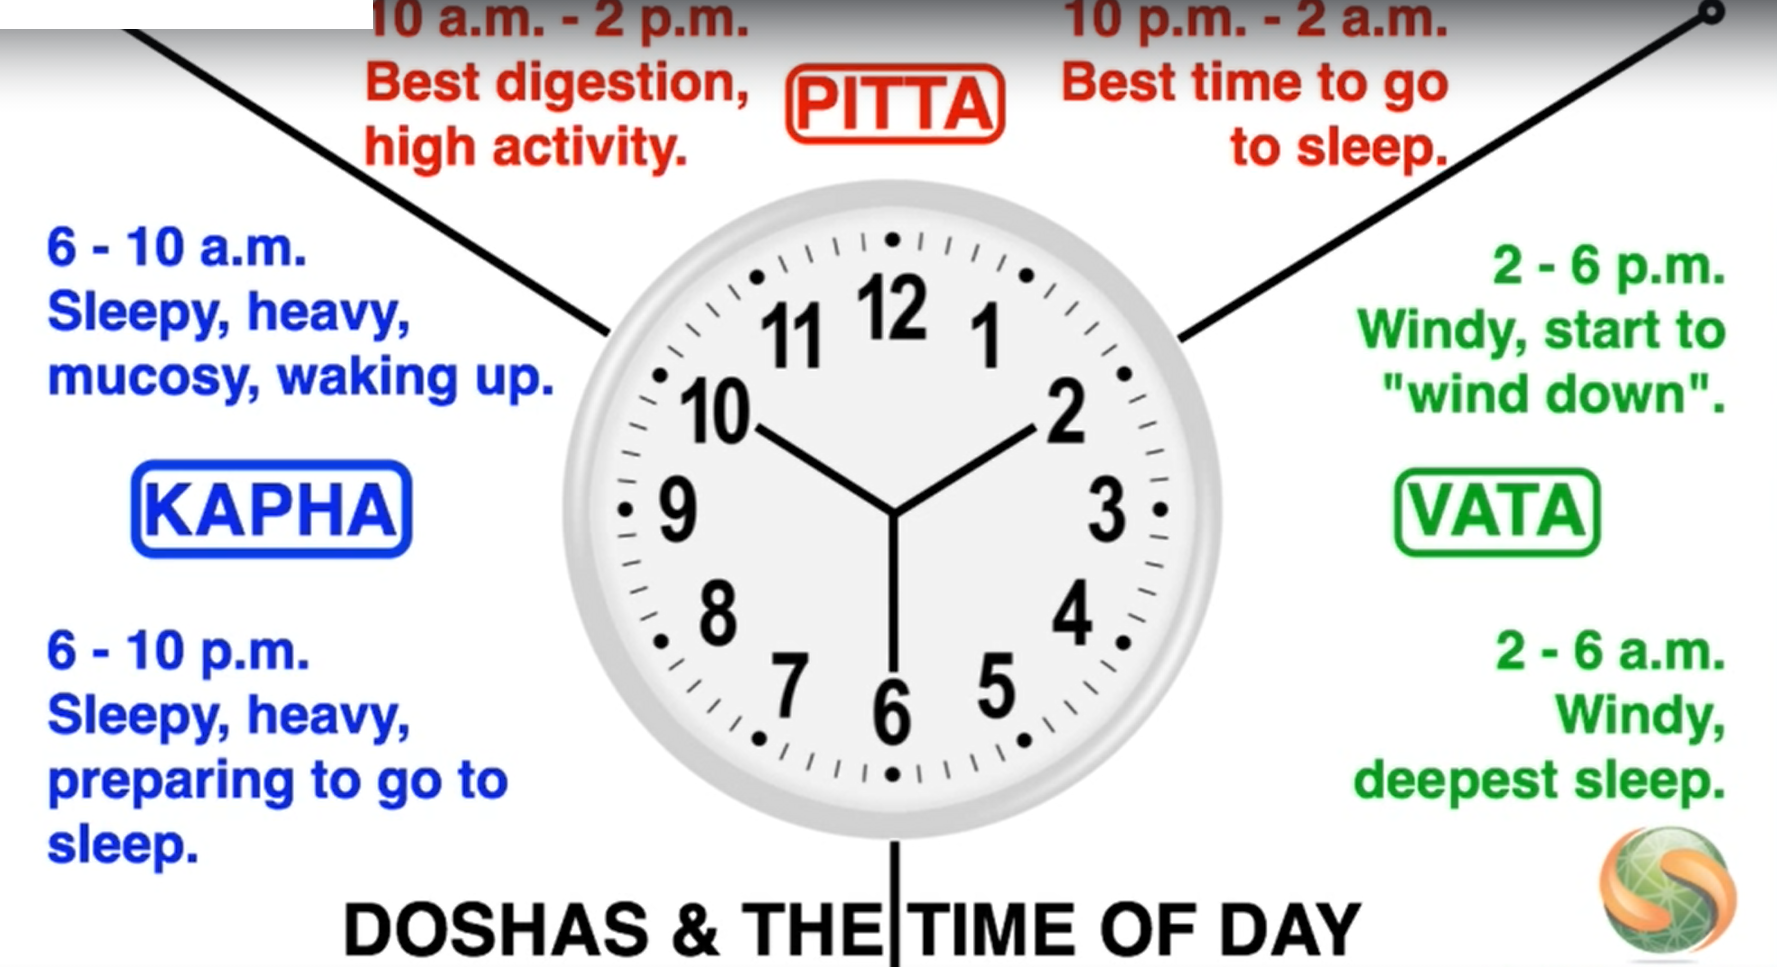
\includegraphics[width=0.7\linewidth,keepaspectratio]{images/ayur3}
\end{center}

{\tiny (Ref: Ayurveda basics, Udemy)}

\end{frame}



%%%%%%%%%%%%%%%%%%%%%%%%%%%%%%%%%%%%%%%%%%%%%%%%%%%%%%%%%%%
\begin{frame}[fragile]\frametitle{Mind Types}
Based on advantages (गुण)

	\begin{itemize}
	\item  रजस Activity/unsteady state of mind
	\item तमस  Inertia/lazy state of mind
	\item सत्त्व Clarity/stillness of mind
	\end{itemize}

\end{frame}

%%%%%%%%%%%%%%%%%%%%%%%%%%%%%%%%%%%%%%%%%%%%%%%%%%%%%%%%%%%
\begin{frame}[fragile]\frametitle{प्रकृति vs विकृति}


	\begin{itemize}
	\item प्रकृति is what you are born with, gets decided at the conception.
	\item विकृति is your current state.
	\end{itemize}

\begin{center}
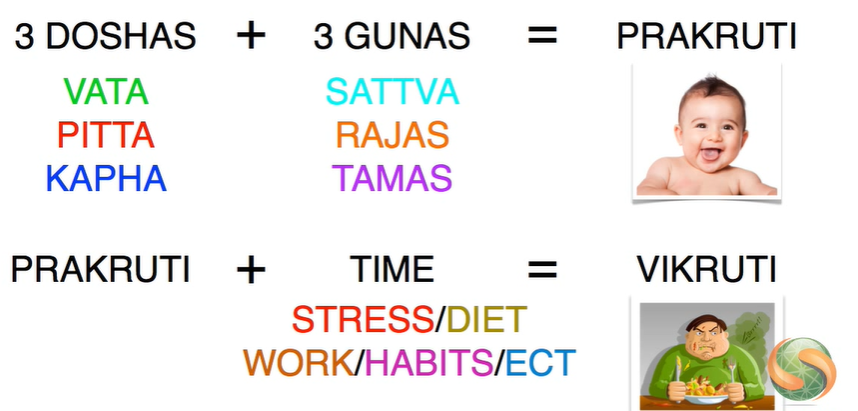
\includegraphics[width=0.7\linewidth,keepaspectratio]{images/ayur4}
\end{center}

{\tiny (Ref: Ayurveda basics, Udemy)}

\end{frame}

%%%%%%%%%%%%%%%%%%%%%%%%%%%%%%%%%%%%%%%%%%%%%%%%%%%%%%%%%%%
\begin{frame}[fragile]\frametitle{7 धातु}

Tissues that bind us together

	\begin{itemize}
	\item  रस Plasma, the nutrient part of blood
	\item रक्त WBCs part of the blood
	\item मांस Muscles
	\item मेद Fats
	\item अस्थि Bones
	\item मज्जा Nerves
	\item शुक्र Male reproduction
	\item अर्थव Female reproduction

	\end{itemize}

\end{frame}

%%%%%%%%%%%%%%%%%%%%%%%%%%%%%%%%%%%%%%%%%%%%%%%%%%%%%%%%%%%
\begin{frame}[fragile]\frametitle{Body Cleansing}
पञ्चकर्म

	\begin{itemize}
	\item  वमन Vomiting, upward movement of कफ
	\item विरेचन Purgation, downward movement of पित्त
	\item नस्य Putting oil/poweder in nose to purify nose and head.
	\item बस्ति Enema, downward movement of वात
	\item रक्त मोक्श Removing toxic blood
	\end{itemize}

\end{frame}


%%%%%%%%%%%%%%%%%%%%%%%%%%%%%%%%%%%%%%%%%%%%%%%%%%%%%%%%%%%
\begin{frame}[fragile]\frametitle{Food Conversion}


\begin{center}
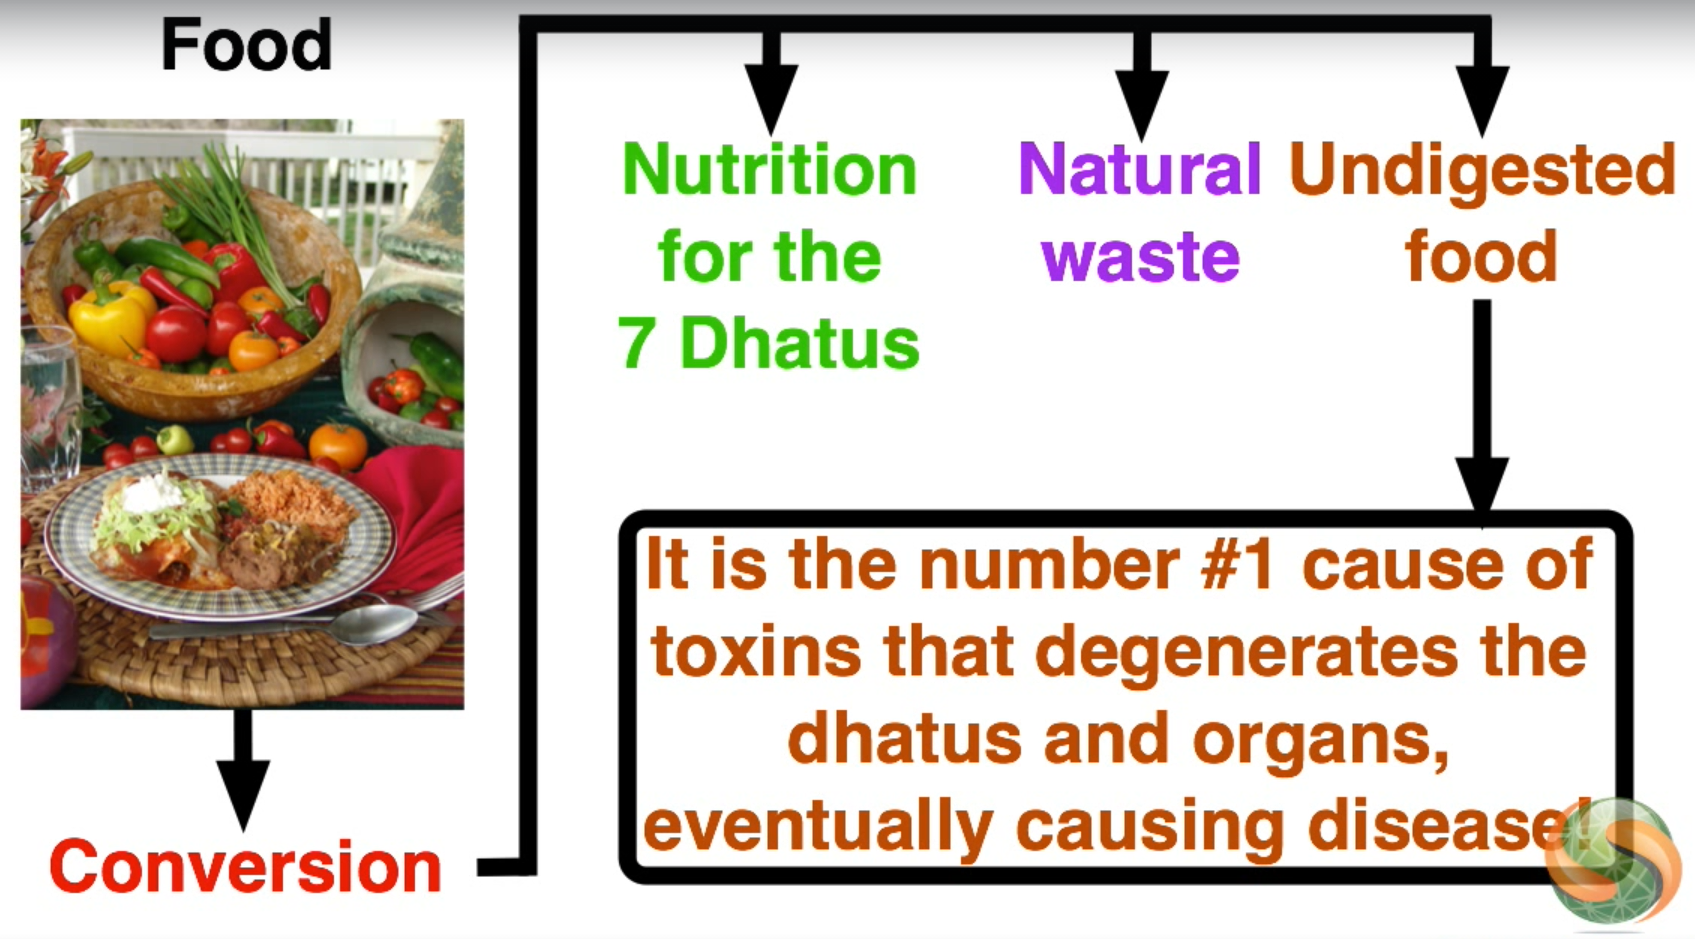
\includegraphics[width=0.7\linewidth,keepaspectratio]{images/ayur5}
\end{center}

{\tiny (Ref: Ayurveda basics, Udemy)}

\end{frame}


%%%%%%%%%%%%%%%%%%%%%%%%%%%%%%%%%%%%%%%%%%%%%%%%%%%%%%%%%%%
\begin{frame}[fragile]\frametitle{Sources Referred}

Many sources have been used in the preparation of this content. Some of the salient ones are listed below:

	\begin{itemize}
	\item Udemy: Discover your mind-body type
	\item Udemy: Ayurveda basics	
	\end{itemize}

\end{frame}


% %%%%%%%%%%%%%%%%%%%%%%%%%%%%%%%%%%%%%%%%%%%%%%%%%%%%%%%%%%%
% \begin{frame}[fragile]\frametitle{International Yoga Day (IYD)}
% 21st June, every year. Why this day/date?

   % \begin{columns}
    % \begin{column}[t]{0.4\linewidth}
	
% \begin{center}
% 
\includegraphics[width=0.5\linewidth,keepaspectratio]{images/yog16}
% \end{center}


    % \end{column}
    % \begin{column}[t]{0.6\linewidth}
		% \begin{center}
		% \textit{``By proclaiming 21 June as the International Day of Yoga, the General Assembly has recognized the holistic benefits of this timeless practice and its inherent compatibility with the principles and values of the United Nations.'' -    Ban Ki-moon (United Nations Secretary-General)}
	% \end{center}

    % \end{column}
  % \end{columns}

% \end{frame}

